

\documentclass[accentcolor=tud9c,9.5pt,nochapname,bigchapter,paper=a5report]{tudreport}


\usepackage{mathtools}
\usepackage[pdftex,bookmarks=true]{hyperref}

\usepackage{lscape}
\usepackage{hyperref}
\usepackage{graphicx}
\usepackage{trfsigns}


\DeclareMathSizes{9.5}{9.5}{7}{7}
\DeclareMathSizes{10}{10}{7}{7}
\DeclareMathSizes{11}{11}{8}{8}
\begin{document}

\def\Var{{\rm Var}\,}
\def\E{{\rm E}\,}
\def\freq{{(e^{j\omega})}\,}


\title{Digital Signal Processing}
\subtitle{Formulary}
\subsubtitle{Author: Daniel Thiem - studium@daniel-thiem.de\\Version 0.1 - 10.02.2013}

\maketitle
\newpage
\thispagestyle{plain}
\mbox{}
\tableofcontents


\numberwithin{equation}{chapter}
\section*{Preface}
This formulary is based on the formulary of the course Stochastic Signals and Systems,
 which can be found here \url{https://github.com/Tyde/stosigsysfs/blob/master/document.pdf?raw=true}.
If you find any errors or have any ideas for improvement, mail me at studium@daniel-thiem.de
 or file an issue at !GITHUBLINK. The \LaTeX{}  source code is
online on !GITHUBLINK and can be improved and extended.

\chapter{Digital Processing of Continous-Time Signals}
\section{Periodic Sampling}
Basic principles of sampling and transforming signals can be found in the Stochastic Signals and Systems formulary
\subsection{Reconstruction of Band-Limited Signals}
Assume, that $H_r(j\Omega)$ and $h_r(t)$ are the frequency and time responses for an ideal low pass filter where 
$x(n)$ is the input signal. Then the output will be
\begin{equation}
	x_r(t) = \sum\limits_{n=-\infty}^{\infty} x(n)h_r(t-nT)
\end{equation}
Because the filter is assumed to be ideal, its impulse response is given by:
\begin{equation}
	h_r(t)=\frac{\sin(\pi t/T)}{\pi t/T}
\end{equation}
where T is the sampling interval that should fulfil the Nyquist condition $\Omega_s > 2 \Omega_B$
\subsection{Discrete-time Processing of Continous-Time Signals}
To process a continous-time signal $x_c(t)$ with digital signal processing techniques, the following setup is used:\\
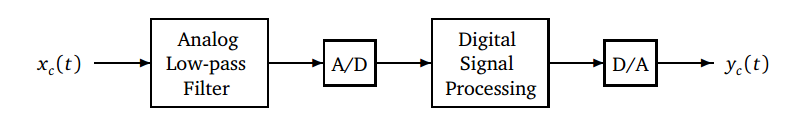
\includegraphics[width=\textwidth]{images/dsp_setup.png}

\chapter{Filter Design}
\section{Digital Filters}
Let $x(n)$ and $y(n) , n=0\pm 1,\ldots$ be the input and the output of the system.  
Linear time-invariant discrete-time systems can be characterized 
 by linear constant coefficient difference equations of the following type, where $\max(N-1,M)$ is the order:
 \begin {equation}
 \sum\limits_{k=0}^{M}a_ky(n-k)= \sum\limits_{r=0}^{N-1} b_r x(n-r)
 \end{equation}
\subsection{Finite Impulse Response (FIR) filter}
If $M=0$ then the impulse response of the filter is finite so that:
\begin{subequations}
\begin{align}
y(n) &= \frac{1}{a_0}\sum\limits_{k=-\infty}^{\infty}b_r x(n-k) \\
\text{comparison with } &\text{the convolution sum yields} \notag \\
h(n) &= \begin{cases}
b_n/a_n, &n=0,\ldots,N-1\\
0, &\text{otherwise}
\end{cases}
\end{align}
\end{subequations}

\subsection{Linear Phase Filters}
A digital filter can be described as linear phase filter if $H\freq$ can be expressed as:
\begin{equation}
	H\freq = H_M\freq e^{-j\omega \alpha}
\end{equation} 
with $H_M\freq$ real and $\alpha$(group delay) constant 

\subsubsection{Generalized linear phase system} \label{genLPS}
A Linear phase system with:
\begin{equation}
	H\freq = H_M\freq e^{-j\omega \alpha + j\beta}
\end{equation}
has to meet the condition:
\begin{equation} 
	\sum\limits_{n=-\infty}^{\infty} h(n)\sin[\omega (n-\alpha )+\beta] = 0 \forall \omega \in \mathbb{R}
\end{equation}

\subsection {Linear Phase FIR Filters}
Applying the condition for generalized linear phase systems (\ref{genLPS}) to the FIR Filters yields two possible causal FIR Systems:
\begin{subequations}
\begin{align}
h(n) &= \begin{cases}
h(N-1-n)	&,0\leq n \leq N-1 \\
0			&,\text{otherwise} 
\end{cases} \\
H\freq &= H_e\freq e^{-j\omega (N-1)/2}
\end{align}
\end{subequations}
{\center and}
\begin{subequations}
\begin{align}
h(n) &= \begin{cases}
-h(N-1-n)	&,0\leq n \leq N-1 \\
0			&,\text{otherwise} 
\end{cases} \\
H\freq &= H_o\freq e^{-j\omega (N-1)/2+j\pi /2}
\end{align}
\end{subequations}

\subsection {FIR Filter Types}
The linear phase FIR filters have been classified into 4 Types:

\begin{itemize}
  \item {\bf Type I} \quad symmetric impulse response and N is odd
  \item {\bf Type II}\quad symmetric impulse response and N is even
  \item {\bf Type III}\quad antisymmetric impulse response and N is odd
  \item {\bf Type IV}\quad antisymmetric impulse response and N is even
\end{itemize}

\subsubsection {Type I linear phase filter}
$N$ is odd and the impuls response is symmetric. $\beta=0$ 
\begin{subequations}
\begin{align}
	h(n)&=h(N-1-n) \quad 0\leq n \leq N-1 \\
	H\freq &= e^{-j\omega \frac{N-1}{2}}\left[{\sum\limits_{k=0}^{(N-1)/2} a(k)\cos(\omega k)}\right]\\
	&\quad\text{where}\notag\\
	a(0)=h\left(\frac{N-1}{2}\right) \text{ and } a(k)&=2h\left(\frac{N-1}{2}-k\right), \quad\quad k=1,2,\ldots,(N-1)/2 \notag
\end{align}
\end{subequations}

\subsubsection {Type II linear phase filter}
$N$ is even and the impuls response is symmetric. $\beta=0$ 
\begin{subequations}
\begin{align}
	h(n)&=h(N-1-n) \quad 0\leq n \leq N-1 \\
	H\freq &= e^{-j\omega \frac{N-1}{2}}\left\{{\sum\limits_{k=1}^{N/2} b(k)\cos\left[\omega \left(k-\frac{1}{2}\right)\right]}\right\}\\
	&\quad\text{where}\notag\\
	b(k)&=2h[N/2-k], \quad\quad k=1,2,\ldots,N/2 \notag
\end{align}
\end{subequations}

\subsubsection {Type III linear phase filter}
$N$ is odd and the impuls response is antisymmetric. $\beta=\pi/2$ 
\begin{subequations}
\begin{align}
	h(n)&=-h(N-1-n) \quad 0\leq n \leq N-1 \\
	H\freq &= je^{-j\omega \frac{N-1}{2}}\left[{\sum\limits_{k=1}^{(N-1)/2} c(k)\sin(\omega k)}\right]\\
	&\quad\text{where}\notag\\
	c(k)&=2h[(N-1)/2-k], \quad\quad k=1,2,\ldots,(N-1)/2 \notag
\end{align}
\end{subequations}

\subsubsection {Type IV linear phase filter}
$N$ is even and the impuls response is antisymmetric. $\beta=\pi/2$ 
\begin{subequations}
\begin{align}
	h(n)&=-h(N-1-n) \quad 0\leq n \leq N-1 \\
	H\freq &= je^{-j\omega \frac{N-1}{2}}\left\{{\sum\limits_{k=1}^{N/2} d(k)\sin\left[\omega \left(k-\frac{1}{2}\right)\right]}\right\}\\
	&\quad\text{where}\notag\\
	d(k)&=2h[N/2-k], \quad\quad k=1,2,\ldots,N/2 \notag
\end{align}
\end{subequations}

\section {Filter Specficaion}
Non-ideal Filters have one or more pass-bands($\omega_p$), 
transition-bands(between $\omega_p$ and $\omega_s$) and stop-bands($\omega_s$). 
For the pass- and the stop- band, a tolerance
$\alpha_i$ has to be specified. Therefore a low-pass filter would have the following specification:
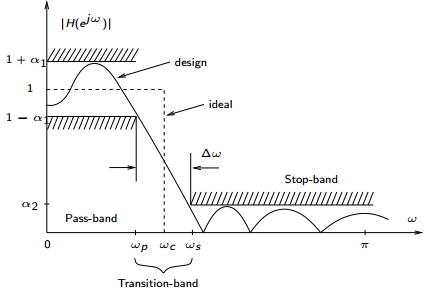
\includegraphics[width=\textwidth]{images/filter_spec.png}


\chapter{Miscellaneous}
\section{Useful mathematical equations}
\subsection{Geometric series}
\begin{equation}
\sum\limits_{n=0}^{N-1} q^n = \frac{1-q^N}{1-q} \quad \text{for} \quad|q|<1
\end{equation} 

\subsection{Conversion from Geometric series to trigonometric fraction}
Let $\frac{1-q^{N}}{1-q}$ be with $q = e^{-j\omega}$
\begin{equation}
\frac{1-e^{-jN\omega}}{1-e^{-j\omega}} = e^{-j\omega \frac{N-1}{2}}\frac{\sin\left(\frac{N}{2}\omega\right)}{\sin\left(\frac{\omega}{2}\right)}
\end{equation}
\end{document}
